\chapter{Hazard Unit}
\label{Hazard Unit}

The Hazard Unit is used to detect 3 different type of hazard: 
\begin{enumerate} 
    \item Raw Hazard in which the pipeline stall to wait the value to read for the current instruction stalled
    \item Jump Hazard when a jump is in decode and flush the instructions after the jump, waiting the new PC
    \item Branch Hazard when a branch is taken in execution unit , flush the pipeline and put new PC
\end{enumerate}

\begin{figure}[h!]
    \centering
    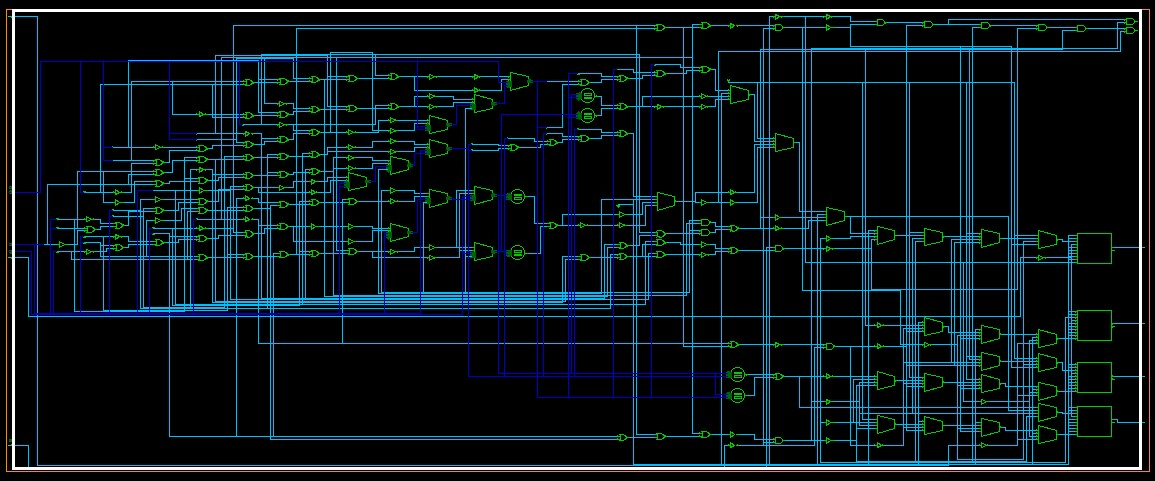
\includegraphics[scale = 0.50]
    {chapters/figures/HU_highlevel}
    \caption{HU}
    \end{figure}

To detect these hazards, the HU works on two processes, executed one after the other.
\begin{enumerate} 
    \item First process: It works on the inputs coming from the CU (IR\_ID,IR\_EX,IR\_MEM). It uses the pipeline and the instruction with its relative opcode (ITYPE,JTYPE,RTYPE) to take the correct registers used (RS1,RS2,RD).This analysis creates also a pipeline of the registers to take into account in which stage the register is, to consider in a correct way raw hazards.
    \item Second process: It is the process used to detect the hazard and it is divided in 2 main part:
    \begin{enumerate}  
        \item In the first part simply there is the detection of a jump/jr/jal in the decode stage (for jr there is also a control on the register used that it could create raw hazard).Also the detection of the branch, in the execute stage, thanks to the result (Branchstatus) given by comp4Branch in the Datapath.In the ifs of jump/jr/jal there is an "AND branchstatus" because of a problem caused by a branch followed by a jump that created an error in which of the two was the correct to take.
        \item Second part: It is used to detect raw hazards between the destination registers in execution-memory with the source registers of the instruction in decode (using the pipeline registers explained before). All the possible combination are considered (ITYPE,RTYPE different source registers and destination registers positions)
    \end{enumerate}
\end{enumerate}

When a hazard is detected a signal called PC\_sel is rised to stop the pc (except for branch) and stalls are implemented in the pipeline with the insertion of NOPs in the correct stages (explained in CU).After the useful stalls, the hazard signal and the PC\_sel go at 0 and the code restarts its correct pipeline.

